% LaTeX template for MICS papers
% To Run:  pdflatex Sample.tex

\documentclass[12pt]{article}

\setlength{\oddsidemargin}{0in}
\setlength{\evensidemargin}{0in}
\setlength{\topmargin}{0in}
\setlength{\headheight}{0in}
\setlength{\headsep}{0in}
\setlength{\textwidth}{6in}
\setlength{\textheight}{9in}
\usepackage[parfill]{parskip}

\usepackage{graphicx} %For jpg figure inclusion
\usepackage{float}
\usepackage{times} %For typeface

\begin{document}
\pagestyle{plain}

\title{Accelerating Biomolecular Nuclear Magnetic Resonance Assignment with A*}

\author{
Joel Venzke, Paxten Johnson, Rachel Davis, John Emmons, Katherine Roth,\\ David Mascharka, Leah Robison, Timothy Urness and Adina Kilpatrick\\
Department of Mathematics and Computer Science\\
Drake University\\
Des Moines, IA\\
email % TODO
}
\date{} 

\maketitle
\thispagestyle{empty}

\section*{\centering Abstract}

Nuclear magnetic resonance (NMR) spectroscopy is a powerful method for studying the three-dimensional structure of molecules such as proteins. The post-genomic era has created the need to gather functional and structural information of unknown proteins encoded by newly discovered genes. Unfortunately, current manual techniques for analyzing NMR datasets can take days to months to assign, and are prone to error. The current goal of this research is to develop an algorithm to automate the process of assigning nontrivial NMR datasets, in an attempt to minimize human error and accelerate a time consuming task.
%
NMR images yield structural information that needs to be analyzed rapidly and accurately. Accurate assignment of nontrivial NMR datasets will provide the necessary framework for continued advancement in the fields of structural biology and proteomics. 
%
The algorithm utilizes A* search to sequence amino acids produced from NMR datasets of proteins. The program is given a set of nodes, each corresponding to a single amino acid in the protein chain, from an input file. Each node is placed in the initial node position of the protein chain. The node that most correctly fits the reference protein chain is used to generate child nodes. Unplaced nodes are sequentially added to the end of a list to create child node lists. The node list with the smallest error is then expanded further. The error is a running total of how well the nodes fit the reference protein chain, coupled with the accuracy of the match of the placed child. This process of assigning the child nodes and calculating costs repeats until every node is placed and the best node list contains the lowest cost of all generated lists. 
%
Assignments of test sets have shown this method can be used to assign NMR datasets, but there remains need for improvement. Research is ongoing as we continue to refine our algorithm. Future goals include adjusting for potentially missing data, sorting nodes into amino acid groups, and testing with larger datasets. Upon completion, this algorithm will allow for great advancements in the areas of structural biology and proteomics. 
\newpage
\setcounter{page}{1}

\section{Introduction}
\label{sub:introduction}
Knowledge of a protein’s structure allows for further understanding of the function of a protein and alterations to its function that can lead to disease. Through the implementation of Nuclear magnetic resonance (NMR) spectroscopy, the structure of molecules, such as proteins, can be studied. However, assigning NMR spectroscopy generates large amounts of data that needs to be assigned. This process can take months to complete and is prone to error. To allow for major advances in structural biology, a faster and more accurate method needs to be developed. Our research focuses on developing an algorithm to automate the assignment process. We hope our attempts can minimize the human error and decrease the time consumption associated with manual assignment , increasing the overall effectiveness of the operation.

\subsection{Nuclear Magnetic Resonance Spectroscopy} % (fold)
\label{sub:nmr}
Several types of NMR variables can be used in the analysis of protein structures. In particular, essential information is provided by the chemical shifts of NMR-active nuclei present in proteins, including hydrogen and isotopes of carbon and nitrogen. The chemical shift is a quantifier for the deviation in the resonant frequency of a nucleus from its value in a structure-free environment, and therefore provides information on the local conformation. Determining the chemical shifts of all or most of the nuclei in a biomolecule is the first step in determining its structure. An important set of chemical shifts in a protein are those corresponding to the nuclei in the backbone of the protein polypeptide chain, including the nitrogen, attached hydrogen, and the alpha and beta carbon atoms ($C_\alpha$ and $C_{\beta}$) of each residue. These chemical shifts are measured using various three-dimensional NMR experiments, and then matched to the individual residues in the protein in a process called sequential assignment.

A prerequisite of the assignment process is data collection using experiments that can provide connectivities between neighboring residues. For example, the HNCACB experiment identifies the chemical shifts corresponding to the $C_\alpha$ and $C_{\beta}$ nuclei of one residue (residue $i$), as well as the $C_\alpha$ and $C_{\beta}$ chemical shifts of the immediately preceding residue (residue $i -1$). In this experiment, the values corresponding to residue $i$ can usually be distinguished from the ($i -1$) values by their higher intensity. However, ambiguities can arise if the intensities are comparable or if the chemical shift values are overlapping. These ambiguities can be resolved by using additional experiments, such as CBCA(CO) NH, which yields the chemical shifts of the preceding residue only. Using all inter-residue connectivities, a chain of correlations through the protein backbone chemical shifts can be established.  This pattern of sequentially linked chemical shift values reflects the sequential linear arrangement of the individual residues in the protein sequence. The pattern is then matched with the protein sequence, by using the fact that certain residues have characteristic $C_\alpha$ and $C_{\beta}$ chemical shift ranges which uniquely identify them. Thus, each measured chemical shift is assigned to a protein residue, and this information can then be used to infer structural information about the biomolecule.

\section{Assignment Methods} % (fold)
\label{sec:method}

\subsection{Manual Assignment} % (fold)
\label{sub:manual_assignment}
% TODO
add this part
cite our sources

% subsection manual_assignment (end)

\subsection{Our Algorithm} % (fold)
\label{sub:algorithm}
Our algorithm begins by reading in an expected amino acid order and the NMR carbon shift data from a data file. It then changes the amino acids to their expected $C_\alpha$ and $C_{\beta}$ values and stores them in a list that represents the protein chain. Next, the carbon shift values for a single amino acid are placed in a tile. A tile contains the $C_\alpha$ and $C_{\beta}$ values for the amino acid residue $i$ and residue $i-1$. Next, missing data is accounted for. If there are fewer tiles than the number of amino acids in the protein chain, placeholder tiles are generated to make up the difference. Before the search for the best solution begins, the tiles are grouped by the types of amino acids they could represent. The groups were created using the expected $C_\alpha$ and $C_{\beta}$ values shown in Figure~\ref{fig:carbon}. Grouping is done in an attempted to accelerate the assignment process. Tiles that do not match a group are grouped with the placeholder tiles. 

\begin{figure}[H]
\begin{center}
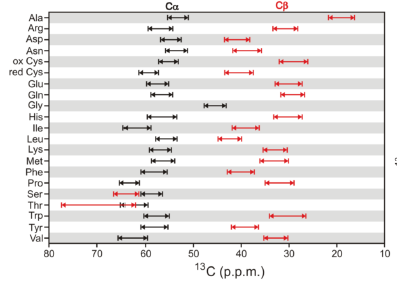
\includegraphics{carbon}
\end{center}
\caption{Expected Carbon Shift Values} % TODO citation
\label{fig:carbon}
\end{figure}

%start search
To start the search, tiles in the placeholder group and tiles of the same amino acid group as the first amino acid in the protein chain are placed in the first position in a node. The tile is then compared to the first amino acid in the protein chain and a cost is generated. The cost is the sum of the cost of placing any previous tiles in the node, how well the current tile matched the corresponding amino acid in the protein chain and how well the tile's residue $i-1$ values match the residue $i$ values of the tile placed before it. All of the generated nodes are placed in a frontier array. 

%continue assignment
The node in the frontier with the lowest cost is removed from the frontier and used to generate child nodes. To generate a child node, a tile is added to the end of the node. A child node is generated for all unplaced tiles that are either in the placeholder group or in the group matching the corresponding amino acid in the protein chain. The cost of placing the tile is then generated.  The child nodes are then added to the frontier, and the process of generating child nodes is repeated. 

%goal state
Once a node has every tile placed, it is said to be in the goal state. The first node that reaches goal state is stored as the current best solution. Every node that achieves goal state is compared to the current best solution. The node with the lowest cost is then saved as the current best solution. 

%solution found
A solution has been found once the current best solution's cost is lower than the cost of any nodes in the frontier. The search is then ended. The algorithm then outputs the cost of the best solution followed by the assigned carbon shift values. 

\section{Conclusions}
\label{sec:conclusions}

\subsection{Results}
\label{sub:results}
Our algorithm has been tested with NMR datasets of varying size from experiments conducted by Dr. Kilpatrick.  When compared to manually assigned data, the algorithm produces the same, optimal ordering of amino acids. Initially, we focused our research on accurate assignment at the cost of speed. Thus, at the start of our research our algorithm was only able to assign smaller datasets with a chain of ten to fifteen amino acids. Shifting our focus to optimizing the algorithm's speed while maintaining the accuracy we had managed to achieve, we were able to improve runtime. With the increased runtime, we were able to correctly assign forty to fifty amino acids. In future research, we plan to test with larger datasets, maximizing speed and efficiency to the point that our algorithm can assign full protein(amino acid?) sequences. We also plan to look into testing datasets with more than a few missing data points to verify that our algorithm correctly places amino acids when given less perfect data.  - TIME FOR DATASETS?

\subsection{Future Goals} % (fold)
\label{sub:future_goals}
In future research, we will look into maximizing speed and efficiency to the point that our algorithm can assign full amino acid sequences. In order to achieve this, we will experiment with  both parallelization (techniques) and machine learning. The latter of these two will assist in optimizing the cost calculation while the former will increase the speed of assignment. We believe these implementations will help our algorithm handle datasets with numerous missing data points, validating our results even when given incomplete data. 
% subsection future_goals (end)

% subsection algorithm (end)
% section method (end)
\bibliographystyle{amc}
\bibliography{Paper}

\end{document}
